\chapter{Graphene}
\label{ch:graphene}
Graphene is one of the most studied materials in history\cite{KatsnelsonBook, Murakami2009, CastroNeto2009a,
Mas-Balleste2011, Rozhkov2016, Han2014, Konschuh2011a, Cooper2012, Sadurni2014}.
Even before its experimental discovery\cite{Novoselov2004, Novoselov2005}
deep research was devoted to it\cite{Wallace1947, Oshima2000, Forbeaux1998, VanBommel1975, Semenoff1984, Haldane1988}.
All the basic properties have been discussed profusely\cite{Cooper2012, Geim2007}, yet, for the shake of completeness I will make a brief recap of all the relevant properties for the rest of this thesis.\\

Graphene consists of a two-dimensional array of carbon, $C$ atoms arranged in a honeycomb lattice like those shown in Fig.~\ref{graphene_structure}~($a-d$)\cite{Ishigami2007}. The honeycomb lattice is not a proper Bravais lattice itself so, in order to describe such a system in terms of Bloch functions, we can choose a wide variety of unit cells and lattice vectors as long as it tessellates the space.
%~~~~~~~~~~~~~~~~~~~~~~~~~~ FIGURE ~~~~~~~~~~~~~~~~~~~~~~~~~%
\begin{figure}[h!]
\centering
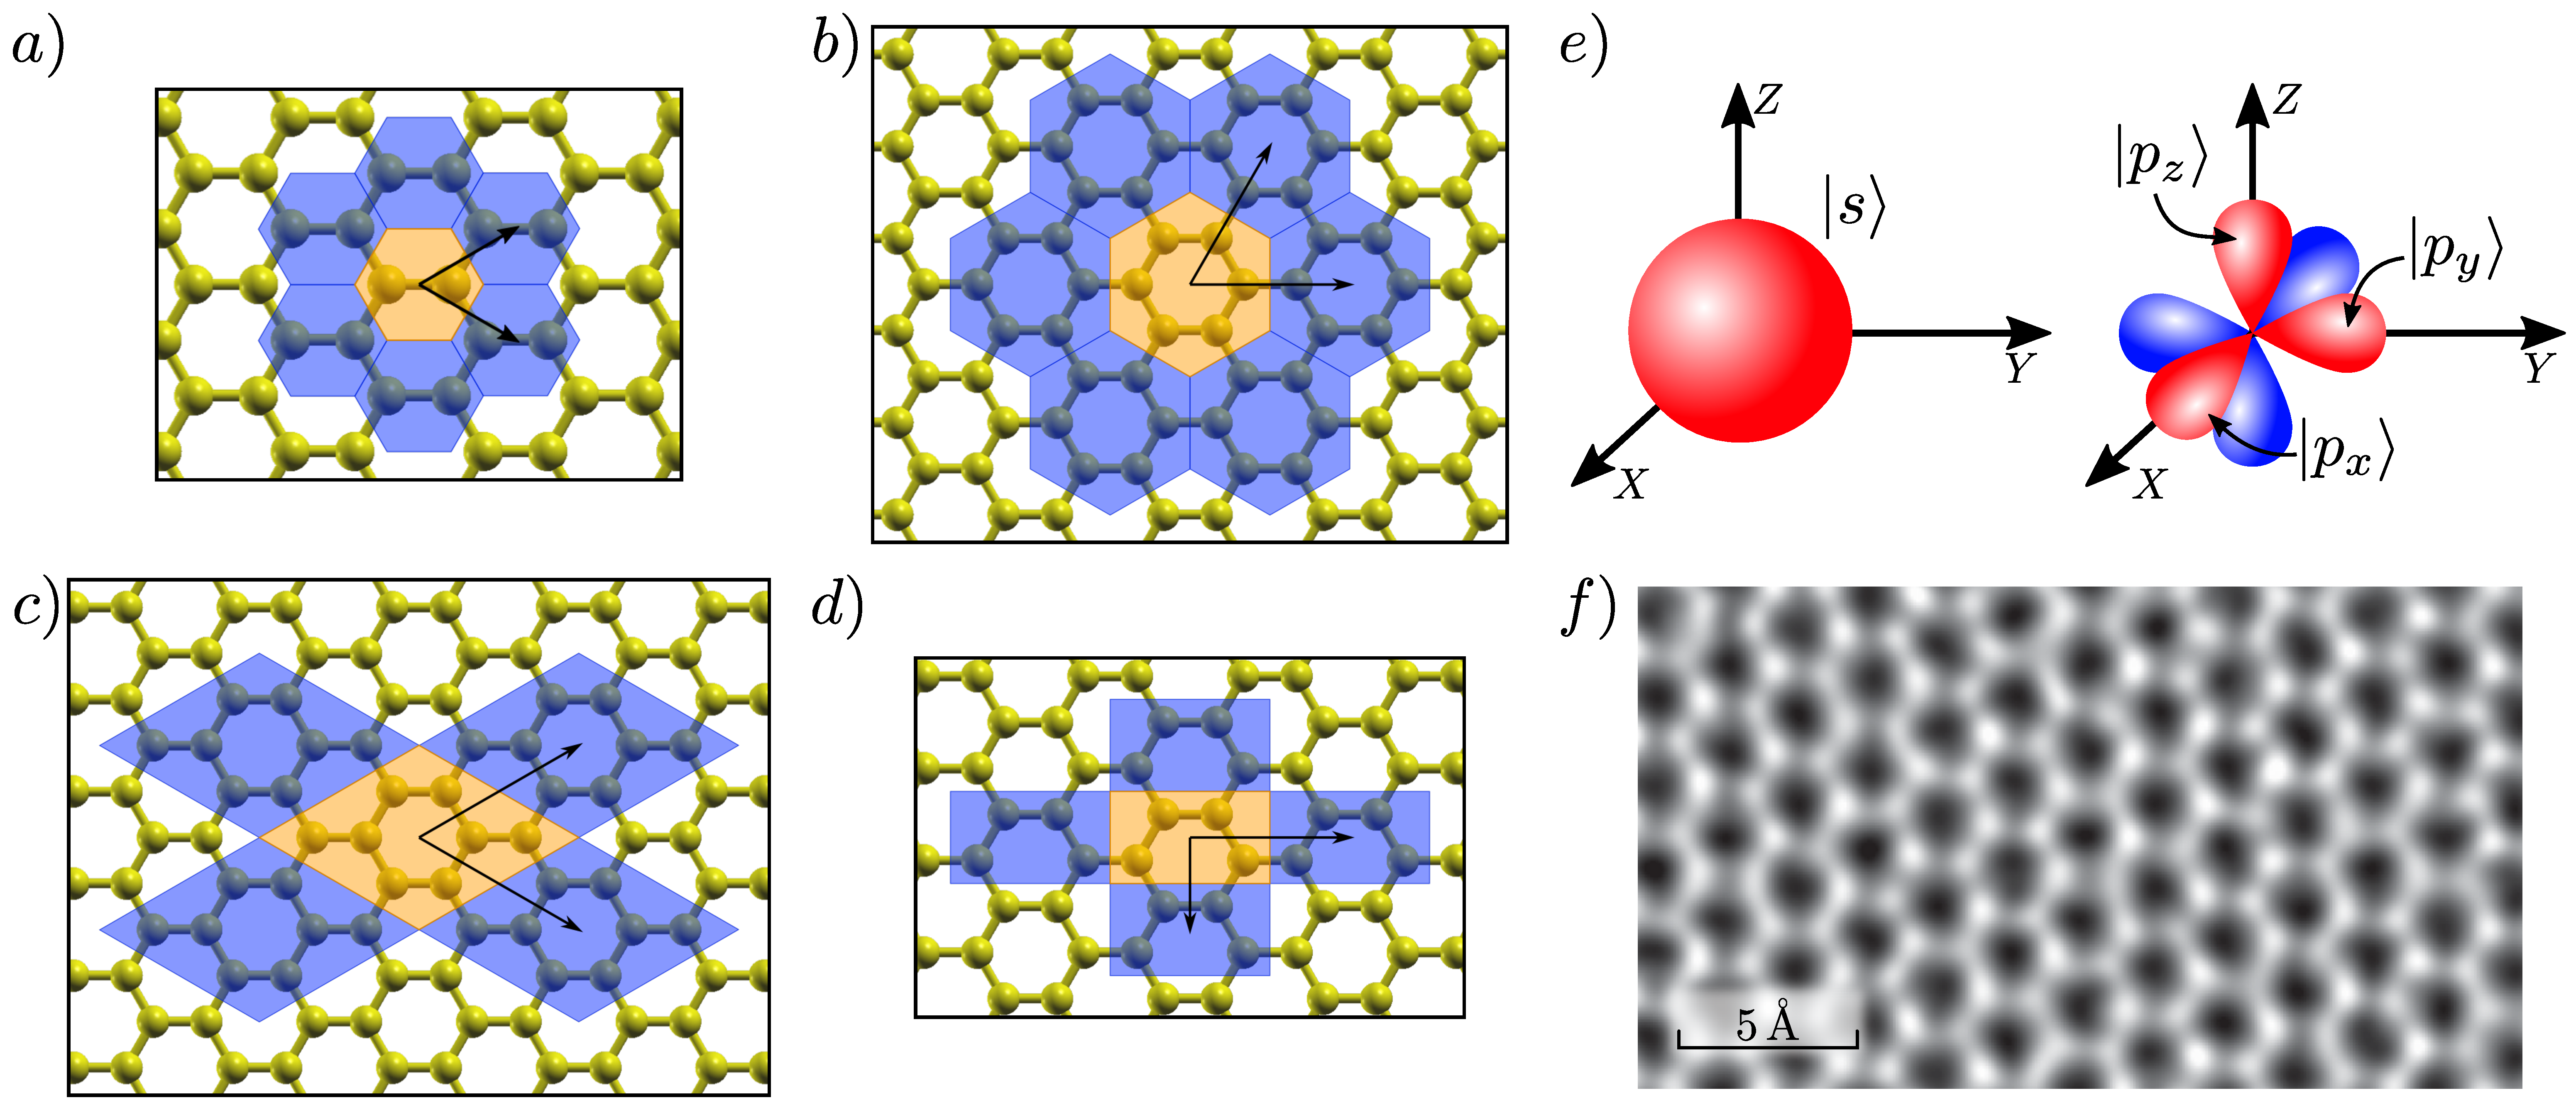
\includegraphics[width=\textwidth]{chapter04/figures/graphene.pdf}
\vspace{-5pt}
\caption{$a-d)$ Graphene atomic structure considering different unit cells and lattice vectors. Notice that not all the descriptions of graphene use a triangular lattice, in fact $d)$ shows graphene as described with a rectangular lattice. The colored regions are the different Wigner-Seitz cells. $e)$ relevant hydrogenic orbitals for the $C$ atom. The $\ket{1s}$ orbital is full and only the $\ket{n=2}$ orbitals will play a role. $f)$ STM image of graphene taken from ref~\cite{Huang2011}}
\label{graphene_structure}
\end{figure}
\FloatBarrier
%~~~~~~~~~~~~~~~~~~~~~~~~~~~~~~~~~~~~~~~~~~~~~~~~~~~~~~~~~~~%
Unless otherwise stated, we will consider that the unstrained atomic distance between carbon atoms is $d_{C-C}=a=\SI{1.4}{\angstrom}$ in accordance with literature\cite{KatsnelsonBook, Cooper2012}. % TODO more biblio
As stated previously the honeycomb lattice is not a Bravais lattice. In orer to describe the basic properties of graphene it the minimal unit cell is the one depicted in Fig.~\ref{graphene_structure}~a), with two atoms in the positions
\begin{equation}
\vec{r}_0 = \tfrac{a}{2}(-1,0,0) \quad;\quad
\vec{r}_1 = \tfrac{a}{2}(1,0,0),
\label{at_pos}
\end{equation}
The lattice vectors that define the Bravais lattice are:
\begin{equation}
\vec{a}_1 = \tfrac{a}{2}\left(3,\sqrt{3},0\right) \quad;\quad
\vec{a}_2 = \tfrac{a}{2}\left(3,-\sqrt{3},0\right)
\label{latt_vec}
\end{equation}

Once the lattice structure is clear, we turn to the atomic properties. Carbon atoms have 6 \acp{el} allocated in five orbitals. The first two \acp{el} are in the $1s$ level, two more in the $2s$ level and finally another two \acp{el} in the $2p$ levels (Fig.~\ref{graphene_structure}~(e)).

Since the orbitals $n=1$ are doubly occupied and far down in energy there is no need to consider them. The $2s$ level is also full, but not so far from the Fermi energy (around $-\SI{-8}{\eV}$), so we will take a look at its importance. The $2p$ orbitals are the closest to the Fermi level, hence they will play a major role in the chemistry of graphene.

We are going to use a \ac{tb} approximation with a basis of localized hydrogenic orbitals. Depending on the physical property that we are interested in we will consider one of two possible basis.
One, considering only one orbital per lattice site:
\begin{equation}
  \mathcal{B}_1 = \left\{\ket{\phi^1_{p_z}}, \ket{\phi^2_{p_z}},\dots, \ket{\phi^n_{p_z}}\right\}
\label{basis1}
\end{equation}
and the other with four orbitals per atom.
\begin{equation}
  \mathcal{B}_4 = \left\{
  \ket{\phi^1_{s}},\ket{\phi^1_{p_x}},\ket{\phi^1_{p_y}},\ket{\phi^1_{p_z}},
  \dots,
  \ket{\phi^n_{s}},\ket{\phi^n_{p_x}},\ket{\phi^n_{p_y}},\ket{\phi^n_{p_z}}
  \right\}
\label{basis4}
\end{equation}
The superscript points out the atom and the subscript shows the corresponding orbital.
% These two basis describe graphene with only one orbital per site, or with four orbitals per site. The reasons why these two descriptions can be used will be shown in the following section %TODO add link

\section{Basic Properties}
\label{sec:graphene_basic_properties}
We are going to start by using a the four orbital basis $\mathcal{B}_4$ described in \eqref{basis4} with the geometry of Fig.~\ref{graphene_structure}~a). Our Hamiltonian will have two atoms and four orbitals per atom, so it will be a $8\times8$ matrix\footnote{we consider now spinless fermions.}

In order to calculate the Hamiltonian matrix we need the ten different hoppings that describe every pair of orbitals ($t_{s-s}$, $t_{s-p_x}$, $t_{s-p_y}$, ...). Nevertheless, the number of parameters necessary can be reduced using the symmetries of the orbitals as shown in the next subsection.


\section{Slater-Koster tight-binding model}
\label{sec:SK}
Generally the hopping parameters are an input in any \ac{tb} model, and usually they are calculated by fitting eigenvalues (and possibly eigenfunctions) obtained from \ac{dft} calculations (the eigenfunctions are often projected to a basis of localized atomic orbitals) or by fitting experimental data to reproduce gaps, orbital components or other relevant physical properties.

As a system grows complex, more and more parameters are needed to describe it, nevertheless since the number of different orbitals is finite, one could expect that not every parameter is completely independent from the others.


The \ac{sk} approximation\cite{Slater1954} takes into account the symmetry of the atomic orbitals to reduce the number of parameters needed since some of them are related by rotations or other symmetry operations.
This idea is depicted in Fig.~\ref{complex} where we can see that the hoppings $t_{p_{z},p_{x}}$ and $t_{p_{z},p_{y}}$ are in fact equivalent since one can be obtained as a rotation of the other.
%~~~~~~~~~~~~~~~~~~~~~~~~~~ FIGURE ~~~~~~~~~~~~~~~~~~~~~~~~~%
\begin{figure}[h!]
  \centering
  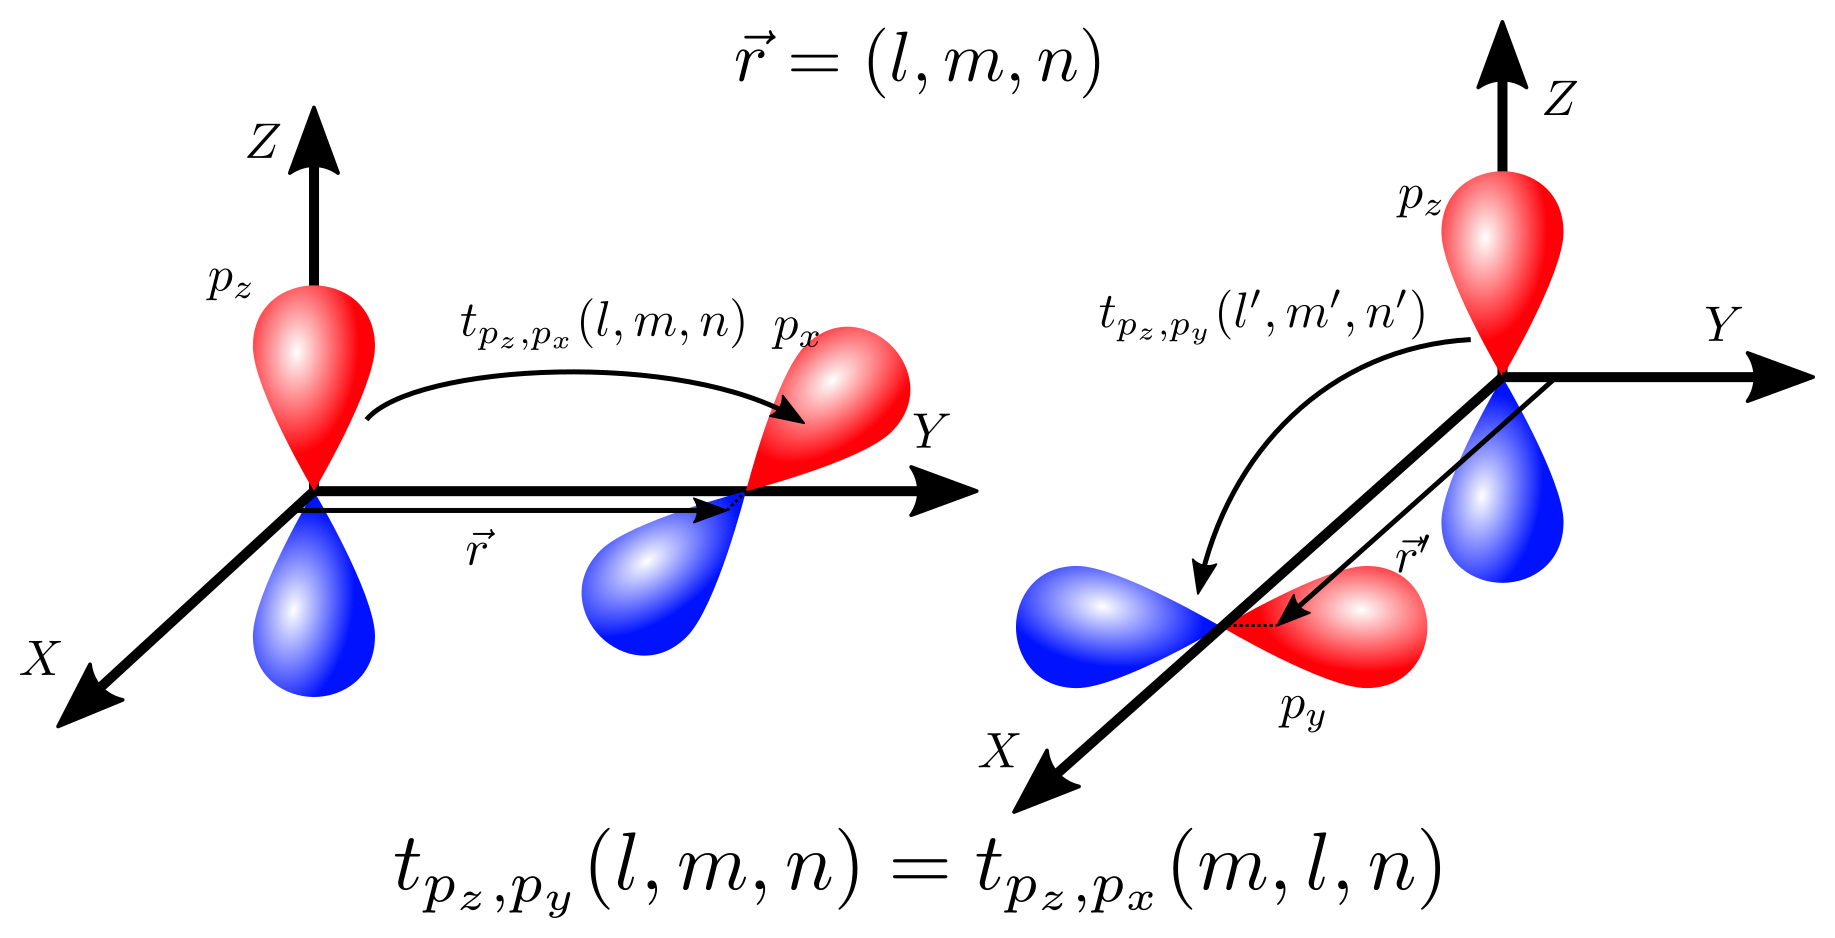
\includegraphics{chapter04/figures/complex.png}
  \vspace{-5pt}
  \caption{Relation between $t_{p_{z},p_{x}}$ and $t_{p_{z},p_{y}}$ hopping. In this case we need not only to rotate each orbital but also the position of the atoms, but it is clear that one hopping can be calculated as a $\pi/2$ clockwise rotation along the Z axis of the other.}
  \label{complex}
\end{figure}
\FloatBarrier
%~~~~~~~~~~~~~~~~~~~~~~~~~~~~~~~~~~~~~~~~~~~~~~~~~~~~~~~~~~~%
If we define the unitary vector $\hat{r} = \vec{r}/|\vec{r}|$ and call its components $l$, $m$, $n$, ($\hat{r}=(l,m,n)$) we can see that
\begin{equation}
  t_{p_{z},p_{x}} (l,m,n) = t_{p_{z},p_{y}}(m,l,n)
\end{equation}
notice that the change in the arguments is equivalent to perform a rotation of the vector $\vec{r}$ of $-\pi/2$ around the $Z$ axis, as shown in Fig.~\ref{complex}.


Even though  this transformations can be deduced by sheer ``brute force'', there is a more general approach that allows the decomposition of any arbitrary hopping in a finite set of bond types.

The easiest way to visualize this decomposition is to consider an arbitrary hopping between two orbitals separated by an arbitrary vector $\vec{r}$, as depicted in the right panel of Fig.~\ref{bonds}. % TODO add letter to panels
Such a hopping can be decomposed in two contributions depending on the relative orientation of the orbitals, namely $\pi$-bonds and $\sigma$-bonds (see Fig.~\ref{bonds}).
%~~~~~~~~~~~~~~~~~~~~~~~~~~ FIGURE ~~~~~~~~~~~~~~~~~~~~~~~~~%
\begin{figure}[h!]
\centering
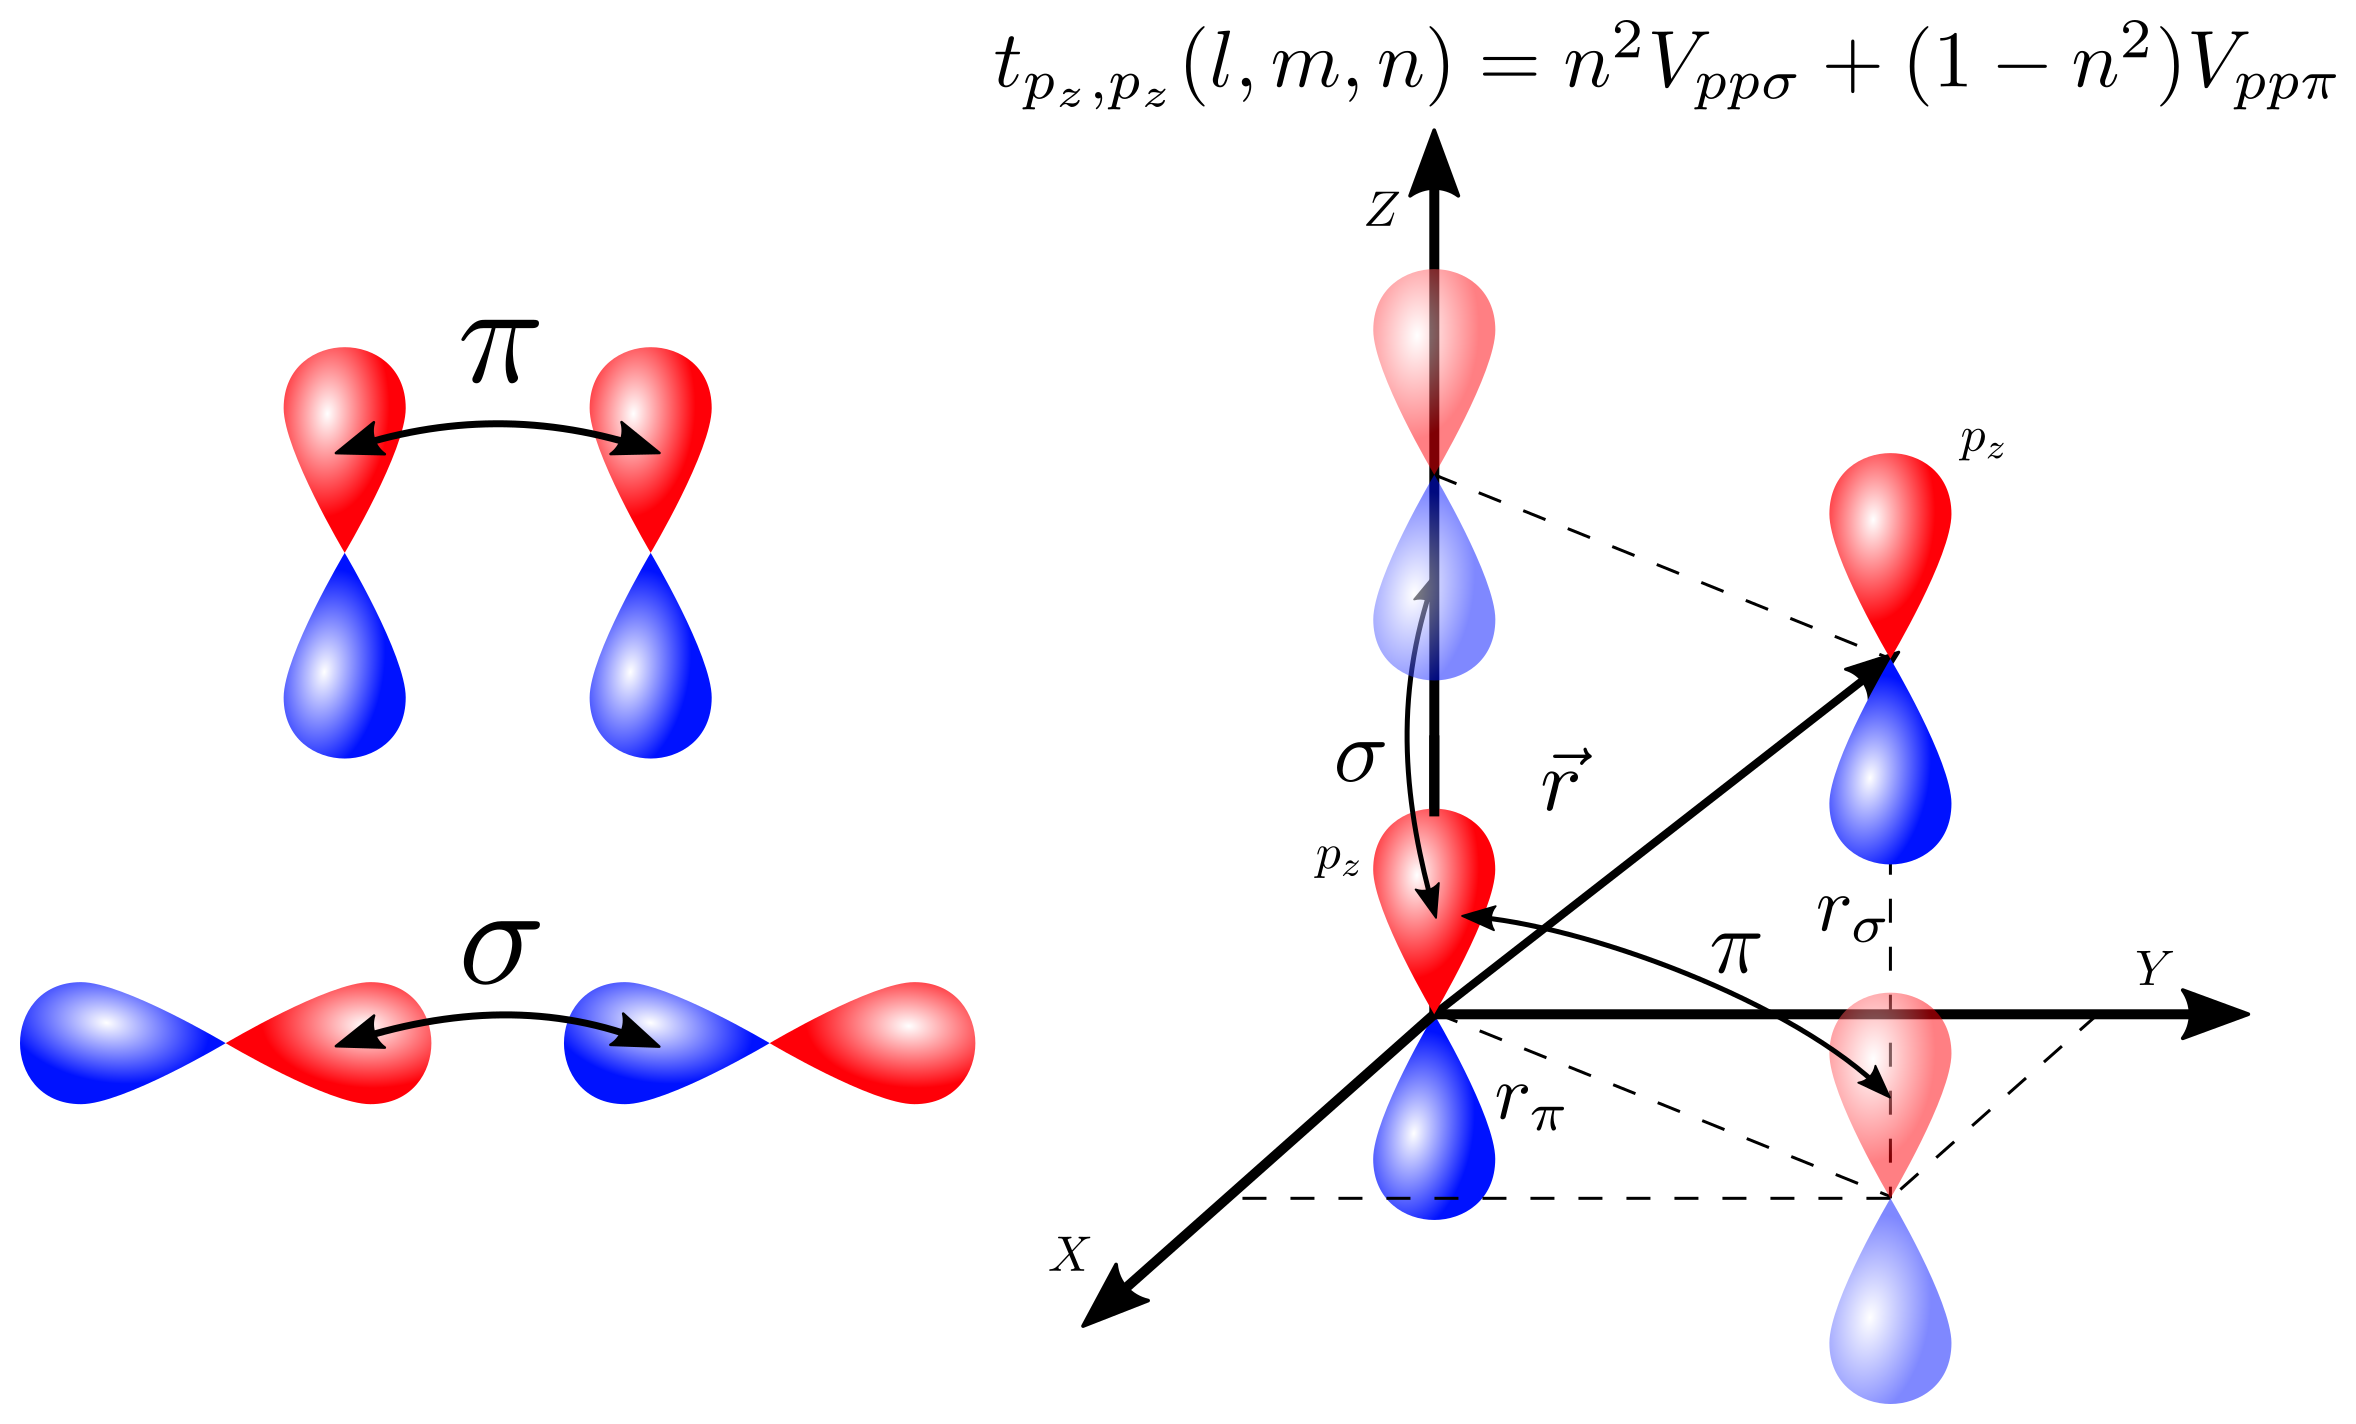
\includegraphics{chapter04/figures/bonds.png}
\vspace{-5pt}
\caption{$a)$ Only two different types of bonds between $p$ orbitals. $b)$ Simplification of the \ac{sk} hopping parameter by decomposing the hopping into its $\sigma$ and $\pi$ component, in this case it is easy to see that the hopping from any $p_{z}$ orbital to another one that in the $XY$ plane will be purely a $\pi$ bond.}
\label{bonds}
\end{figure}
\FloatBarrier
%~~~~~~~~~~~~~~~~~~~~~~~~~~~~~~~~~~~~~~~~~~~~~~~~~~~~~~~~~~~%
% TODO somewhere else? % We can notice in Fig.~\ref{bonds} that in the case of pristine graphene all the in-plane $p_z$-$p_z$ hoppings will be purely $\pi$ bonds, while the other $s$-$p$ hoppings will be $\sigma$ bonds.\\
Let us consider the two orbitals as $p_z$ for simplicity and without any loss of generality. If the two orbitals were aligned along



In the \ac{sk} approximation the atomic distances are encoded in the magnitude of the bonds, $V_{ss\sigma}$, $V_{sp\sigma}$, $V_{pp\sigma}$, $V_{pp\pi}$ (we will call them simply \ac{sk} parameters for short). The coefficients ($l$, $m$, $n$) in the analytic formulas (see appendix~\ref{SKhoppings}) are the responsible for capturing the symmetries arising both form the orbitals and the atomic structure.\\
%XXX Add SK formulas?

This decoupling of magnitude and direction in the hoppings provides a simple model able to capture the effects of geometric deformations, strain and any symmetry (breaking) in the atomic structure. For instance the effect of buckling in graphene is easily captured by this model.\blue{bands, bands with buckling,...}
Bismuth \cite{Liu1995}

\red{explain better}
The effect due to a reduction/increase of the hopping would be included by modifying the \ac{sk} parameters, yet the dependence of this parameters with the interatomic distance is not always easy to calculate.\\

At the end of the day the \ac{sk} approximation results in a reduction of the parameters needed to describe the hoppings in the system. For example, in a system with all the $s$, $p$ and $d$ orbitals (9 types of orbitals) we would expect 36 parameters to describe all the different hoppings, but within the \ac{sk} approximation we would only need 10 parameters.\\


The main drawback for the \ac{sk} model is to actually obtain the \ac{sk} parameters. In fact it is not guaranteed (at all) that for any given system a set of \ac{sk} parameters should exist.
Knowing that this approximation is based upon the symmetry of the atomic orbitals it is expected that for systems where the atomic orbitals are heavily hybridized this description will not suffice.

\red{Discussion limits, covalent, deformation, localized orbitals}



\section{Physical properties of Graphene}
The \ac{sk} parameters used for graphene are:
\begin{equation}
  V_{ss\sigma}= \SI{-7.76}{\eV} \quad;\quad
  V_{sp\sigma}= \SI{8.16}{\eV} \quad;\quad
  V_{pp\sigma}= \SI{7.48}{\eV} \quad;\quad
  V_{pp\pi}= \SI{-2.7}{\eV}
\label{sk_params}
\end{equation}

\subsection{Bands}
Here some bands with \ac{sk}, maybe include bismuth, \ac{bn}, Zeeman, SOC...
%~~~~~~~~~~~~~~~~~~~~~~~~~~ FIGURE ~~~~~~~~~~~~~~~~~~~~~~~~~%
\begin{figure}[h!]
\centering
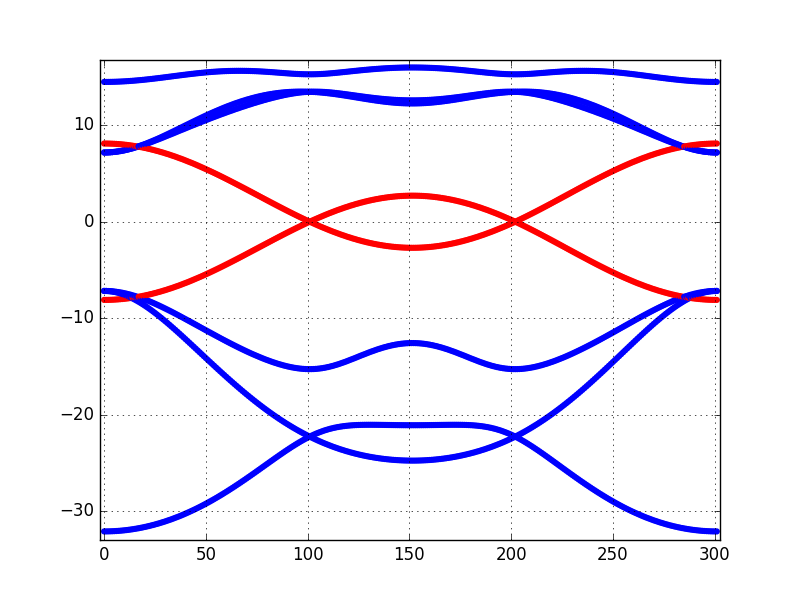
\includegraphics{chapter04/figures/graphene_bands.png}
\vspace{-5pt}
\caption{Graphene bands in the \ac{sk} approximation, with $s$, $p_x$, $p_y$, $p_z$ orbitals for the $C$ atoms. The color denote the $p_z$ component of each state. It can be seen that the $p_z$ orbital are decoupled from the rest of the orbitals and at low energy they are enough to describe the system}
\label{Gbands}
\end{figure}
\FloatBarrier
%~~~~~~~~~~~~~~~~~~~~~~~~~~~~~~~~~~~~~~~~~~~~~~~~~~~~~~~~~~~%
Figure~\ref{Gbands} show the graphene band structure along the $\Gamma,K,K',\Gamma$ path when 4 orbitals per Carbon atom are used, hence the our basis is \eqref{basis4}. In the \ac{tb} approximation any eigenstate of the Hamiltonian will be expressed as a combination of the states of the basis, the color in the band structure is proportional to the expectation value of the $p_z$ projector operator,$\mathcal{O}_{p_z}$,
\begin{equation*}
  \text{color} = \bra{\psi}\mathcal{O}_{p_z}\ket{\psi}
\end{equation*}
where
 \begin{equation*}
   \ket{\psi} = \sum_i c_i\ket{\phi_i} \qquad
   \text{for} \quad\ket{\phi_i}\in\mathcal{B}_4
 \end{equation*}



\subsection{Low energy regime}
Notice that the bands close to the Fermi Energy ($E=0$) only have $p_z$ component, this is due to the mirror symmetry of the $p_z$ orbital and the atomic structure of graphene (planar). In fact this decoupling from the rest of the orbitals allows the
Even in the presence of some interactions that, indeed, mix the $p_z$ manifold with other orbitals, the $p_z$ is still the main component of the the low energy spectra.

An example of such a situation is the graphene bilayer, which be studied in detail in chapter~\ref{ch:bilayer}. In this system the $p_z$ and $s$ orbitals of different layers have a finite hopping, nevertheless when we plot the bands %TODO figure of Gbilayer
we see that most of the contribution is still $p_z$ ($>98\%$ for realistic values of the hoppings).



\section{Quantum Spin Hall}
%%%%%%%%%%%%%%%%%%%%%%%%%%%%%%%%%%%%%%%%%%%%%%%%%%%%%%%%%%%%%%%%%%%%%%%%%%%%%%%%
%%%%%%%%%%%%%%%%%%%%%%%%%%%%%%%%%%%%%%%%%%%%%%%%%%%%%%%%%%%%%%%%%%%%%%%%%%%%%%%%
\subsection{Homogeneous multilayers}\label{Homogeneous}

Monolayer graphene consists of a triangular lattice with two atoms per unit cell that leads, in the reciprocal space, to a hexagonal Brillouin zone that hosts Dirac cones in its corners.
When $N$ layers are considered the crystalline structure remains the same, only there will be $2N$ atoms per unit cell. We shall only use the so called Bernal stacking, shown in  Fig.~\ref{Structure}, which is the ground state configuration, according to both \ac{dft} calculations and experimental evidence~\cite{Norimatsu2010,Charlier1994,Charlier1994a}. In Bernal stacked materials an atom from the sublattice $B$($A$) sits on top of an atom belonging to the other sublattice $A$($B$).
For $N=2$ there is only one way to achieve this, but for $N>2$ there are different possible stacking orders. In figure~\ref{Structure} we show the different possibilities for $N\leq4$, with a self-evident notation.

%~~~~~~~~~~~~~~~~~~~~~~~~~~ FIGURE ~~~~~~~~~~~~~~~~~~~~~~~~~%
\begin{figure}[h!]
\centering
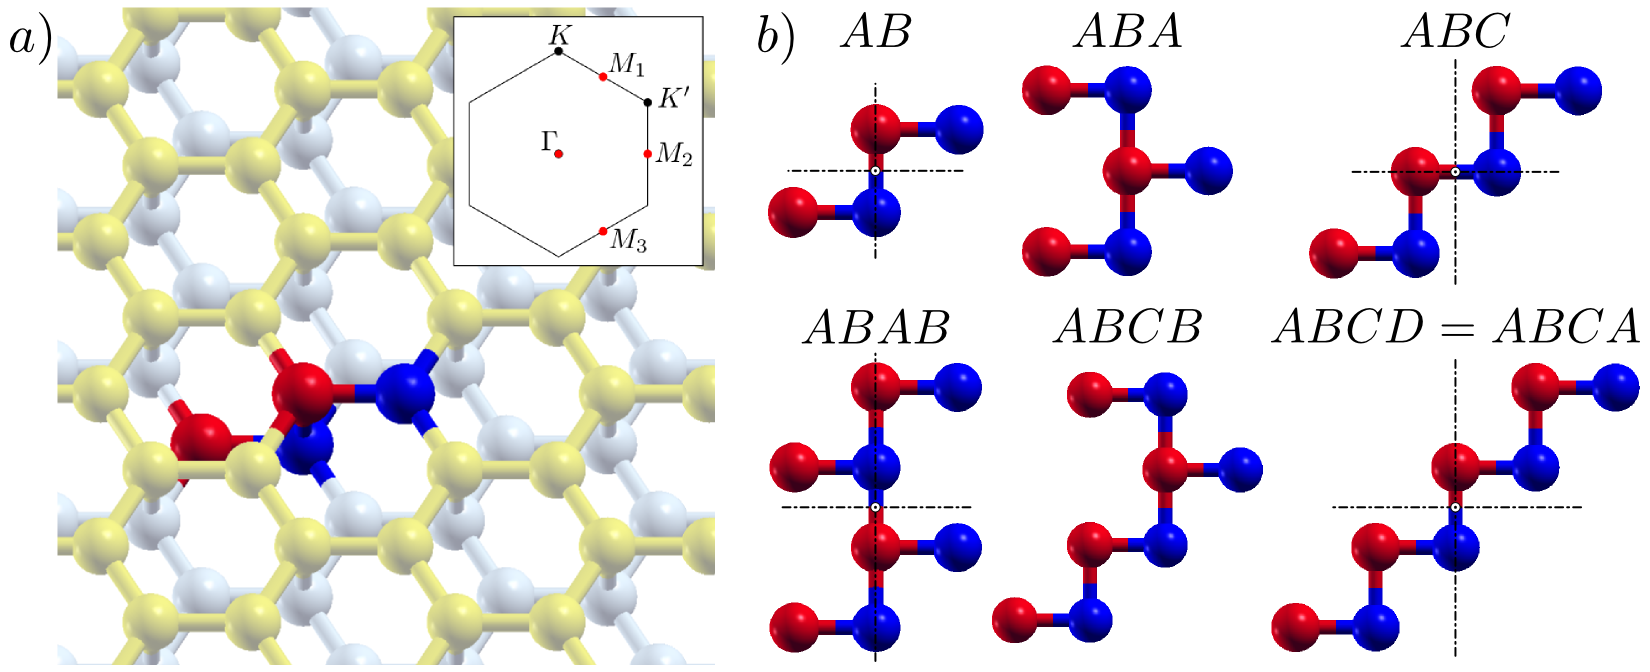
\includegraphics{chapter04/figures/structure.png}
\caption{$a)$ Crystal structure of bilayer graphene system with a highlighted unit cell. Different colors for each layer are used to distinguish the two layers. In the inset the first Brillouin Zone is depicted with the high symmetry points and the Time Reversal Invariant Momenta colored in red. In $b)$ Side view of the unit cells for all the different stackings studied. For the stackings with inversion symmetry the inversion center is shown at the crossing point of the dashed lines. For both figures red and blue denote sublattice.}
\label{Structure}
\end{figure}
%~~~~~~~~~~~~~~~~~~~~~~~~~~~~~~~~~~~~~~~~~~~~~~~~~~~~~~~~~~~%

\subsubsection{The Model}
We describe the multilayers with the following tight-binding Hamiltonian:
\begin{equation}
 H = H_{ML} + \eta H_{inter} + \lambda\vec{L}\cdot\vec{S}
\label{Hamil}
\end{equation}
where $H_{ML}$ and $H_{inter} $ account for the intralayer and interlayer  hoppings, respectively, and the last term is the intra-atomic \ac{soc}. Our tight-binding model is based on four atomic orbitals,  $s$, $p_{x}$, $p_{y}$ and $p_{z}$.
Both the intralayer and interlayer hoppings are described within the \acf{sk} formalism~\cite{Slater1954}. The intralayer hopping parameters are taken from Ref~\cite{Gosalbez-Martinez2011}. In order to study the effect of interlayer coupling, the interlayer terms are scaled by a dimensionless parameter $\eta$. When $\eta=1$, the ratio between interlayer and intralayer $V_{pp\pi}$ in graphene is taken as~\cite{Katsnelson2012} 0.13. Unless otherwise stated, in all our calculations we have $\eta=1$.
Within this model, the dimension of the Hilbert space for the minimal unit cell of the crystal with $N$ layers is $4\times2\times2\times N = 16N$ (4 orbitals per atom, 2 atoms per layer, plus the two possible spin orientations).

Without \ac{soc}, this model reproduces the very well known band structure of graphene ($N=1$) and multilayer graphene $N>1$, that portraits these systems as zero-gap semiconductors. Within this model, \ac{soc} is known to open a gap in the monolayer~\cite{Min2006}  as well as in the bilayer~\cite{Konschuh2012,Guinea2010,Cortijo2010}. In the case of the monolayer graphene the gap is known to be topological. Within this model, the computed value of the gap $\SI{1.46}{\micro\eV}$ when we take a realistic value of the atomic \ac{soc}, $\lambda=\SI{10}{\meV}$. This gap is much smaller than the ones obtained with accurate \ac{dft} calculations~\cite{Konschuh2011a}, in the range of $\sim\SI{30}{\micro\eV}$.
The reason for the discrepancy turns out to be that the mayor contribution to the \ac{soc} gap at the Dirac point comes from the coupling to the higher energy $d$ bands~\cite{Konschuh2012,Konschuh2011a}.
The later is a simple consequence of the fact that \ac{soc} opens a gap in second order in the coupling in the Dirac points when projected over the $p$ band. In comparison, \ac{soc} acts as first order when considering channels involving the $d$ band.
Nevertheless, interlayer hopping may open a first order spin flipping channel in the $p$ manifold, becoming of the same order as the intrinsic spin conserving $d$-level contribution.
These last processes would be the ones missing in the multilayer Kane-Mele model, and should be added for completeness.
In our case, for the sake of simplicity, we will focus on the spin flipping channel, and use a four orbital tight-binding model considering $\lambda$ as a free parameter.

Future work shall focus on the effect of the d-levels in multilayer graphene, which will not be addressed here.

\begin{figure*}
\begin{minipage}{.9\linewidth}
\begin{center}
 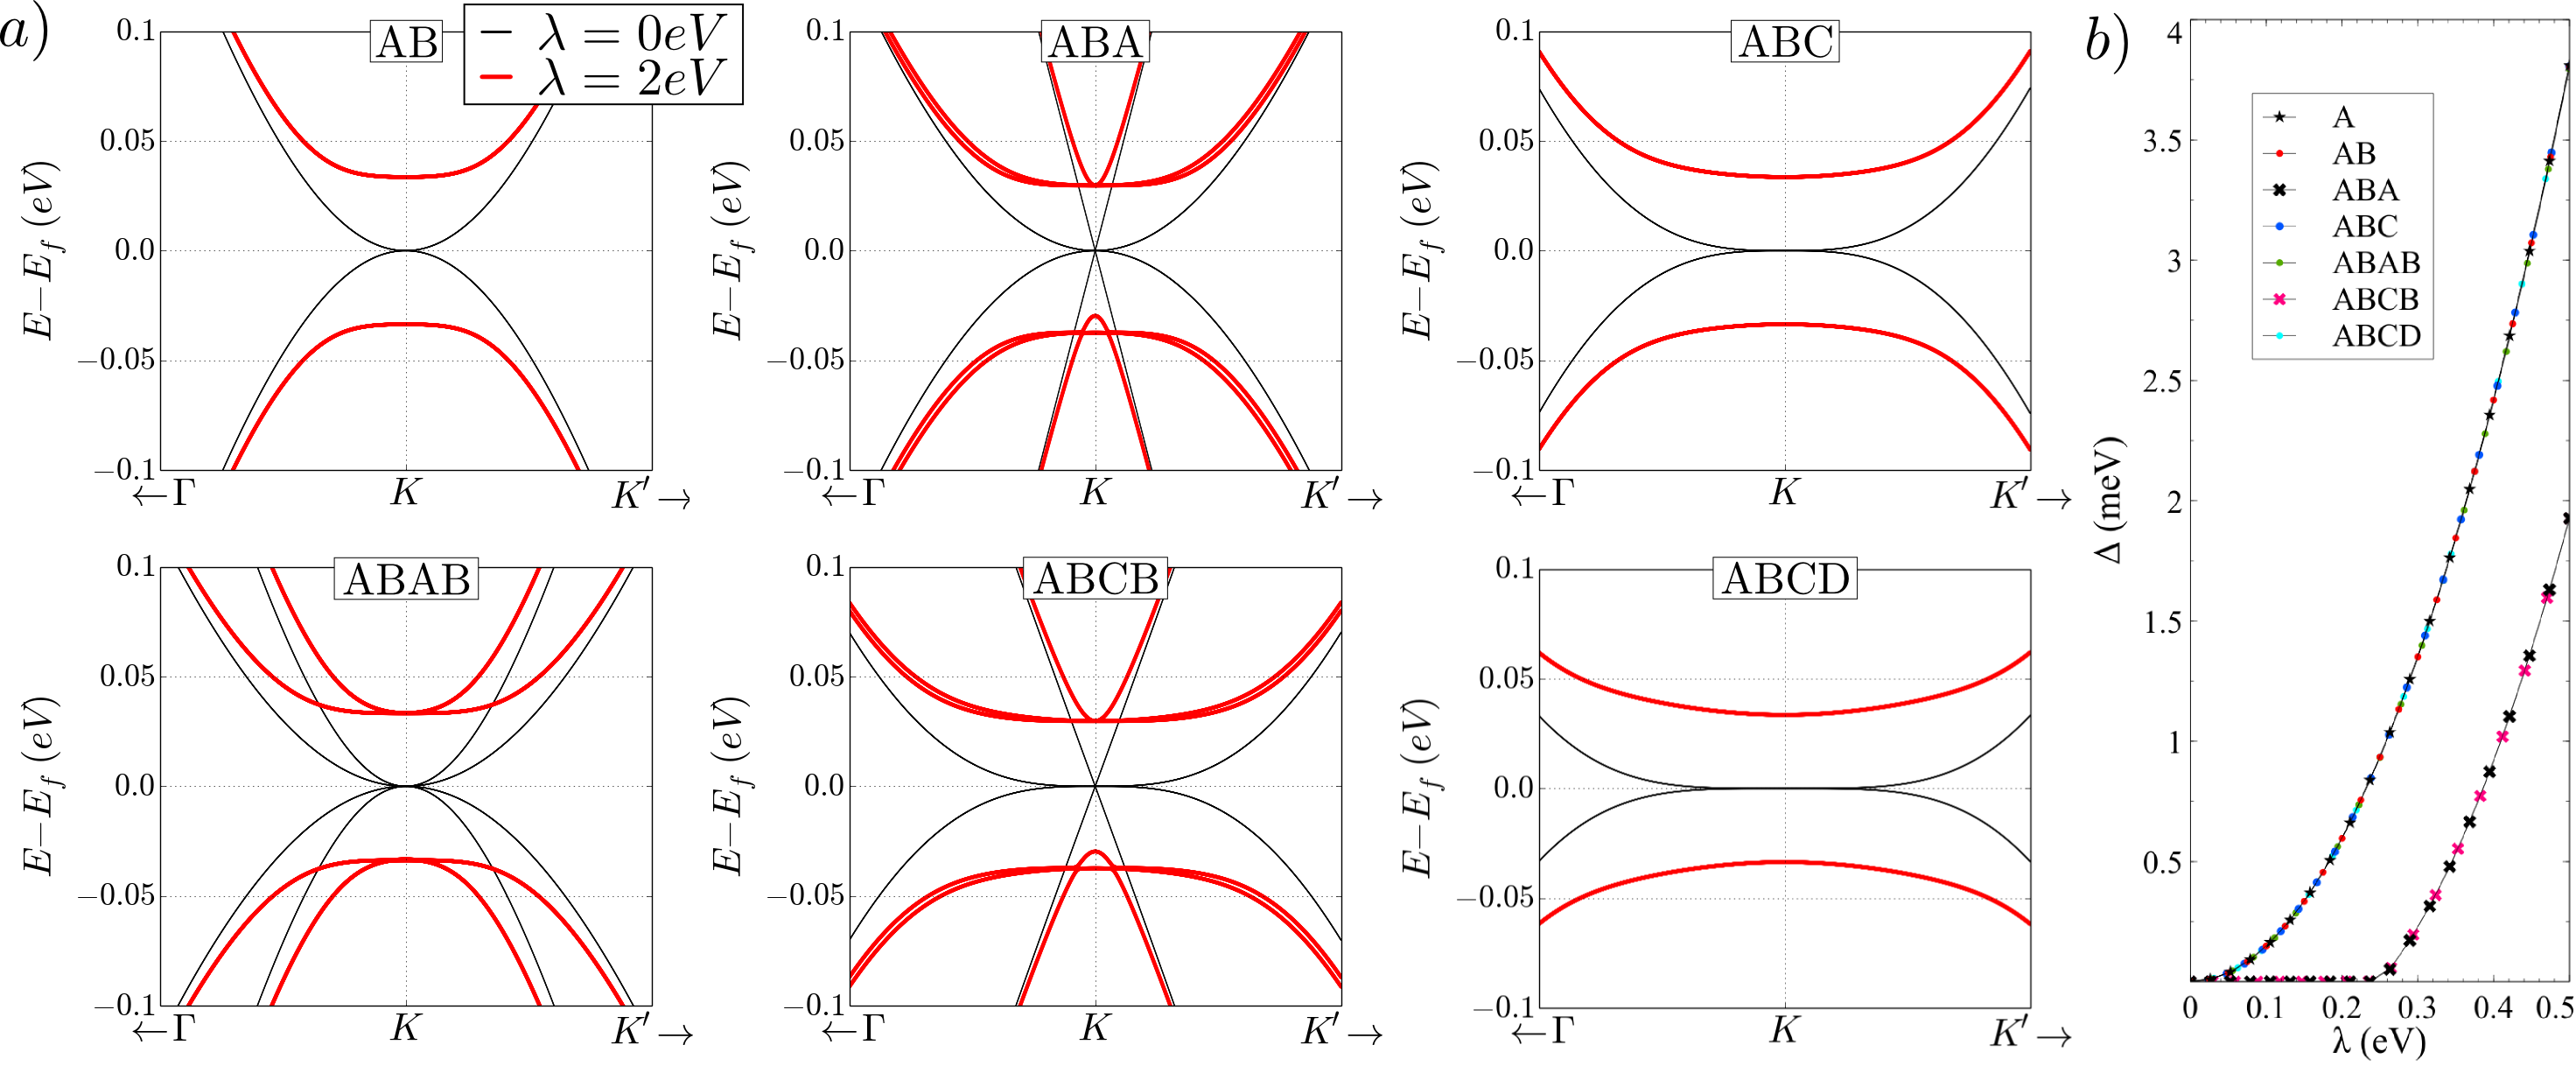
\includegraphics[width=\textwidth]{chapter04/figures/bands.png}
\end{center}
\end{minipage}
\caption{ In $a)$ the band structure close to the $K$ point is shown for all the possible stackings of multilayer graphene with $N = {2,3,4}$. Only when $\lambda \neq 0$ (red line) a gap is opened at the Dirac points.
Note that for $ABA$ and $ABCB$ stackings there are linear bands when $\lambda=0$ that when the \ac{soc} is switched on cause a smaller gap than in the other cases.
In $b)$ the dependence of the gap with the \ac{soc} $\lambda$ is shown. The anomalous behavior for the $ABA$ and $ABCB$ stackings is just due to the linear bands mentioned before.}
\label{Bilayer}
\end{figure*}

The effect of \ac{soc} on the band structure of the multilayers can be summarized in the following points:
\begin{enumerate}
\item \ac{soc}  opens up a gap for all the $N$ stacked layers considered, reproducing the existing results~\cite{Guinea2010} for the case of $N=2$.
Notice that in the case of $ABA$ and $ABCB$ stackings, the system remains gapless until a critical value of $\lambda$.
This peculiarity is related to the non uniform evolution of the SO splitting of the linear and non-linear bands  as shown in figure~\ref{Bilayer}.


\item  The scaling of the gap with $\lambda$ is very similar for monolayer and $N=2,3,4$ multilayers as it is shown in Figure~\ref{Bilayer}. Therefore, it is expected that within this model, the gap opened by the intrinsic \ac{soc} might be as small in multilayers as in monolayers.

\item The magnitude of the band-gap is insensitive to the interlayer coupling. This result is somewhat surprising, since together with atomic \ac{soc} the interlayer coupling opens a spin-flip channel, otherwise missing in the monolayer case.
For the $AB$ bilayer, this can be understood considering the Hamiltonian at the Dirac point, for a given spin flavor. In the basis $\{A_{1},B_{1},A_{2},B_{2}\}$
the low energy Hamiltonian is given by
\begin{equation}
H(K) = \left(\begin{array}{cccc}
\Delta/2 &     0   &    0   &     0 \\
   0   & -\Delta/2 &  \eta t  &     0 \\
   0   &\eta t^{\dagger}&\Delta/2&  0 \\
   0   &     0   &    0   & -\Delta/2
   \end{array}\right)
\end{equation}
where $\Delta$ is the SO gap. When $\eta=0$ this Hamiltonian represents two decoupled monolayers.
For finite $\eta$ the eigenvalues are $E^{1}_{\pm}=\pm\Delta/2$ and $E^{2}_{\pm}=\pm\sqrt{(\eta t)^{2}+(\Delta/2)^{2}}$.
Since $\eta t\gg\Delta$ the gap is still controlled by the $E^{1}$ couple and thereby identical to that of the decoupled monolayers.
As a result, switching on the interlayer coupling does not close the \ac{soc} gap of the monolayer as shown in Figure~\ref{Bilayer}. As a consequence,  the ground state of two decoupled ($\eta=0$) monolayers can be adiabatically connected to the ground state of the bilayer ($\eta=1$).
\end{enumerate}

The last observation leads to the following result: odd $N$ stacked graphene will be quantum spin Hall Insulators, whereas  even $N$ will not. More precisely, for a system of $N$ decoupled monolayers the $Z_{2}$ invariant is:
\begin{equation}
 Z_{2}(N) = \left[Z_{2}(1)\right]^{N}
 \label{trivial}
\end{equation}
Since the gap opened by $\lambda$ remains unaffected when switching on the interlayer coupling $\eta$, the value of $Z_2$ for graphene-like multilayers is also given by equation~\eqref{trivial}.
We have verified that this qualitative behavior remains unchanged when $d$-channels are included in the picture by performing all-electron \ac{dft} calculations. %\cite{elk}.  %XXX CITE ELK
In the realistic low $\lambda$ limit, the gap is controlled by the linear contribution in $\lambda$, namely the $d$-channel. For large SO, the quadratic in $\lambda$ $p$-channel becomes dominant, which corresponds to the situation in which the gap opening is properly captured by the \ac{sk} model.
Thus, by artificially increasing $\lambda$ in a \ac{dft} calculation, it is possible to move from the $d$-dominated to the $p$-dominated SO gap. We have obtained that both limits are adiabatically connected without gap closing, so that the topological properties in the low $\lambda$ limit are the same than in the large $\lambda$ limit.

In the following we verify equation~\eqref{trivial} using two different strategies. In the case of inversion symmetric structures, we compute the $Z_2$ invariant. In all cases, we compute the edge states and check whether they fill the gap, or else.  Independently on how the topological character is obtained, eq.~\eqref{trivial} holds in all the cases.



\subsection{Calculation of the $Z_{2}$ invariant.}
Using the method developed by Fu and Kane in 2007~\cite{Fu2007} for systems with
inversion symmetry it is possible to determine easily its topological character
(the $Z_{2}$ invariant) by calculating the parity of the occupied Bloch wave
functions at the time reversal invariant momenta (TRIMs).

\begin{equation}
\delta_{i} = \displaystyle\prod^{N}_{m=1}\xi_{2m}(\Gamma_{i}) \quad;\quad (-1)^{\nu} = \prod_{i}\delta_{i}
\end{equation}
where $\xi_{2m}$ is the parity eigenvalue of the $2m^{th}$ occupied state at the TRIM $\Gamma_{i}=\{\Gamma,M_{1},M_{2},M_{3}\}$. Using this method the topological character of a system will be determined just by the quantity $(-1)^{\nu}$, resulting that $(-1)^{\nu}=+1$ means trivial topology and $(-1)^{\nu}=-1$ means non trivial topology.
The calculation for the systems with inversion symmetry yields the following results:
\begin{center}
 \begin{tabular}{ c | c c c c c}
              &  A  &  AB & ABC & ABAB & ABCD \\\hline
     $M_{1}$  & $+$ & $+$ & $+$ &  $+$ &  $+$  \\
     $M_{2}$  & $+$ & $+$ & $+$ &  $+$ &  $+$  \\
     $M_{3}$  & $+$ & $+$ & $+$ &  $+$ &  $+$  \\
     $\Gamma$ & $-$ & $+$ & $-$ &  $+$ &  $+$  \\\hline
 $(-1)^{\nu}$ & $-$ & $+$ & $-$ &  $+$ &  $+$
 \end{tabular}
\label{parity}
\end{center}

This guarantees that $A$ and $ABC$  crystals are topological but the bilayers and tetralayers (with inversion symmetry) are not.
%This method cannot be applied to systems without inversion symmetry,  which are addressed in the next section using a different approach.
For systems without inversion symmetry, the calculation of the $Z_{2}$ invariant requires a different approach~\cite{Fu2006, Fukui2005, Fukui2007} that requires a line integral of the Berry curvature over a contour in the Brillouin zone. Instead, we compute the edge states for these systems and invoke the bulk-edge correspondence to address the topological nature of those systems.


\subsection{Edge states}
To confirm equation \eqref{trivial} even for systems without inversion symmetry we look for the presence of gapless edge states.
We consider armchair-terminated  semi-infinite crystals.  Using translation invariance along the direction parallel to the edge, we block-diagonalize  the Hamiltonian of the semi-infinite 2D  crystal in terms of a collection of $k_{||}$ dependent semi-infinite 1D Hamiltonians, as indicated in figure~\ref{Mapping}. The 1D Hamiltonian describes unit cells with $4N$ atoms, where $N$ stands for the number of graphene layers.  The intra-cell terms are denoted by $H_0(k_{||})$ and the inter-cell hoppings by $V(k_{||})$.



\begin{figure}[hbt]
 \centering
  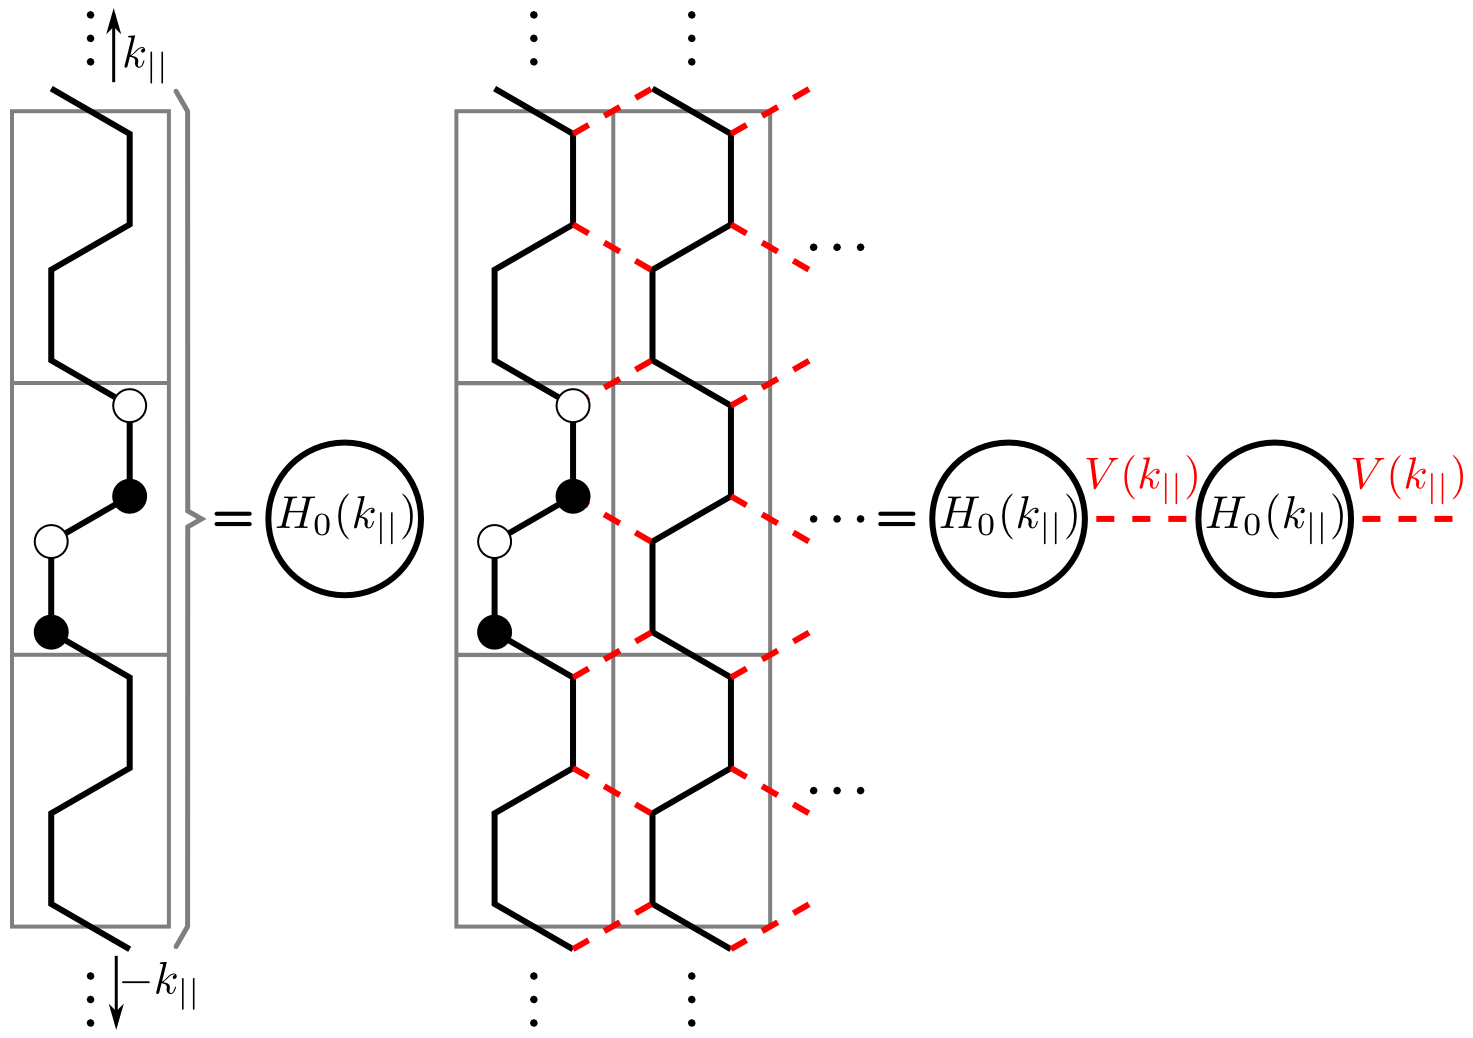
\includegraphics{chapter04/figures/seminfinite.png}
\vspace{-5pt}
\caption{Scheme of the mapping between a semi-infinite crystal and a semi-infinite chain. The coupling between each linear chain (with $k_{||}$ well defined) is introduced by means of a self energy $\Sigma_{R}$.}
\label{Mapping}
\end{figure}

\begin{figure*}
\centering
% \begin{minipage}{.85\linewidth}
% \begin{center}
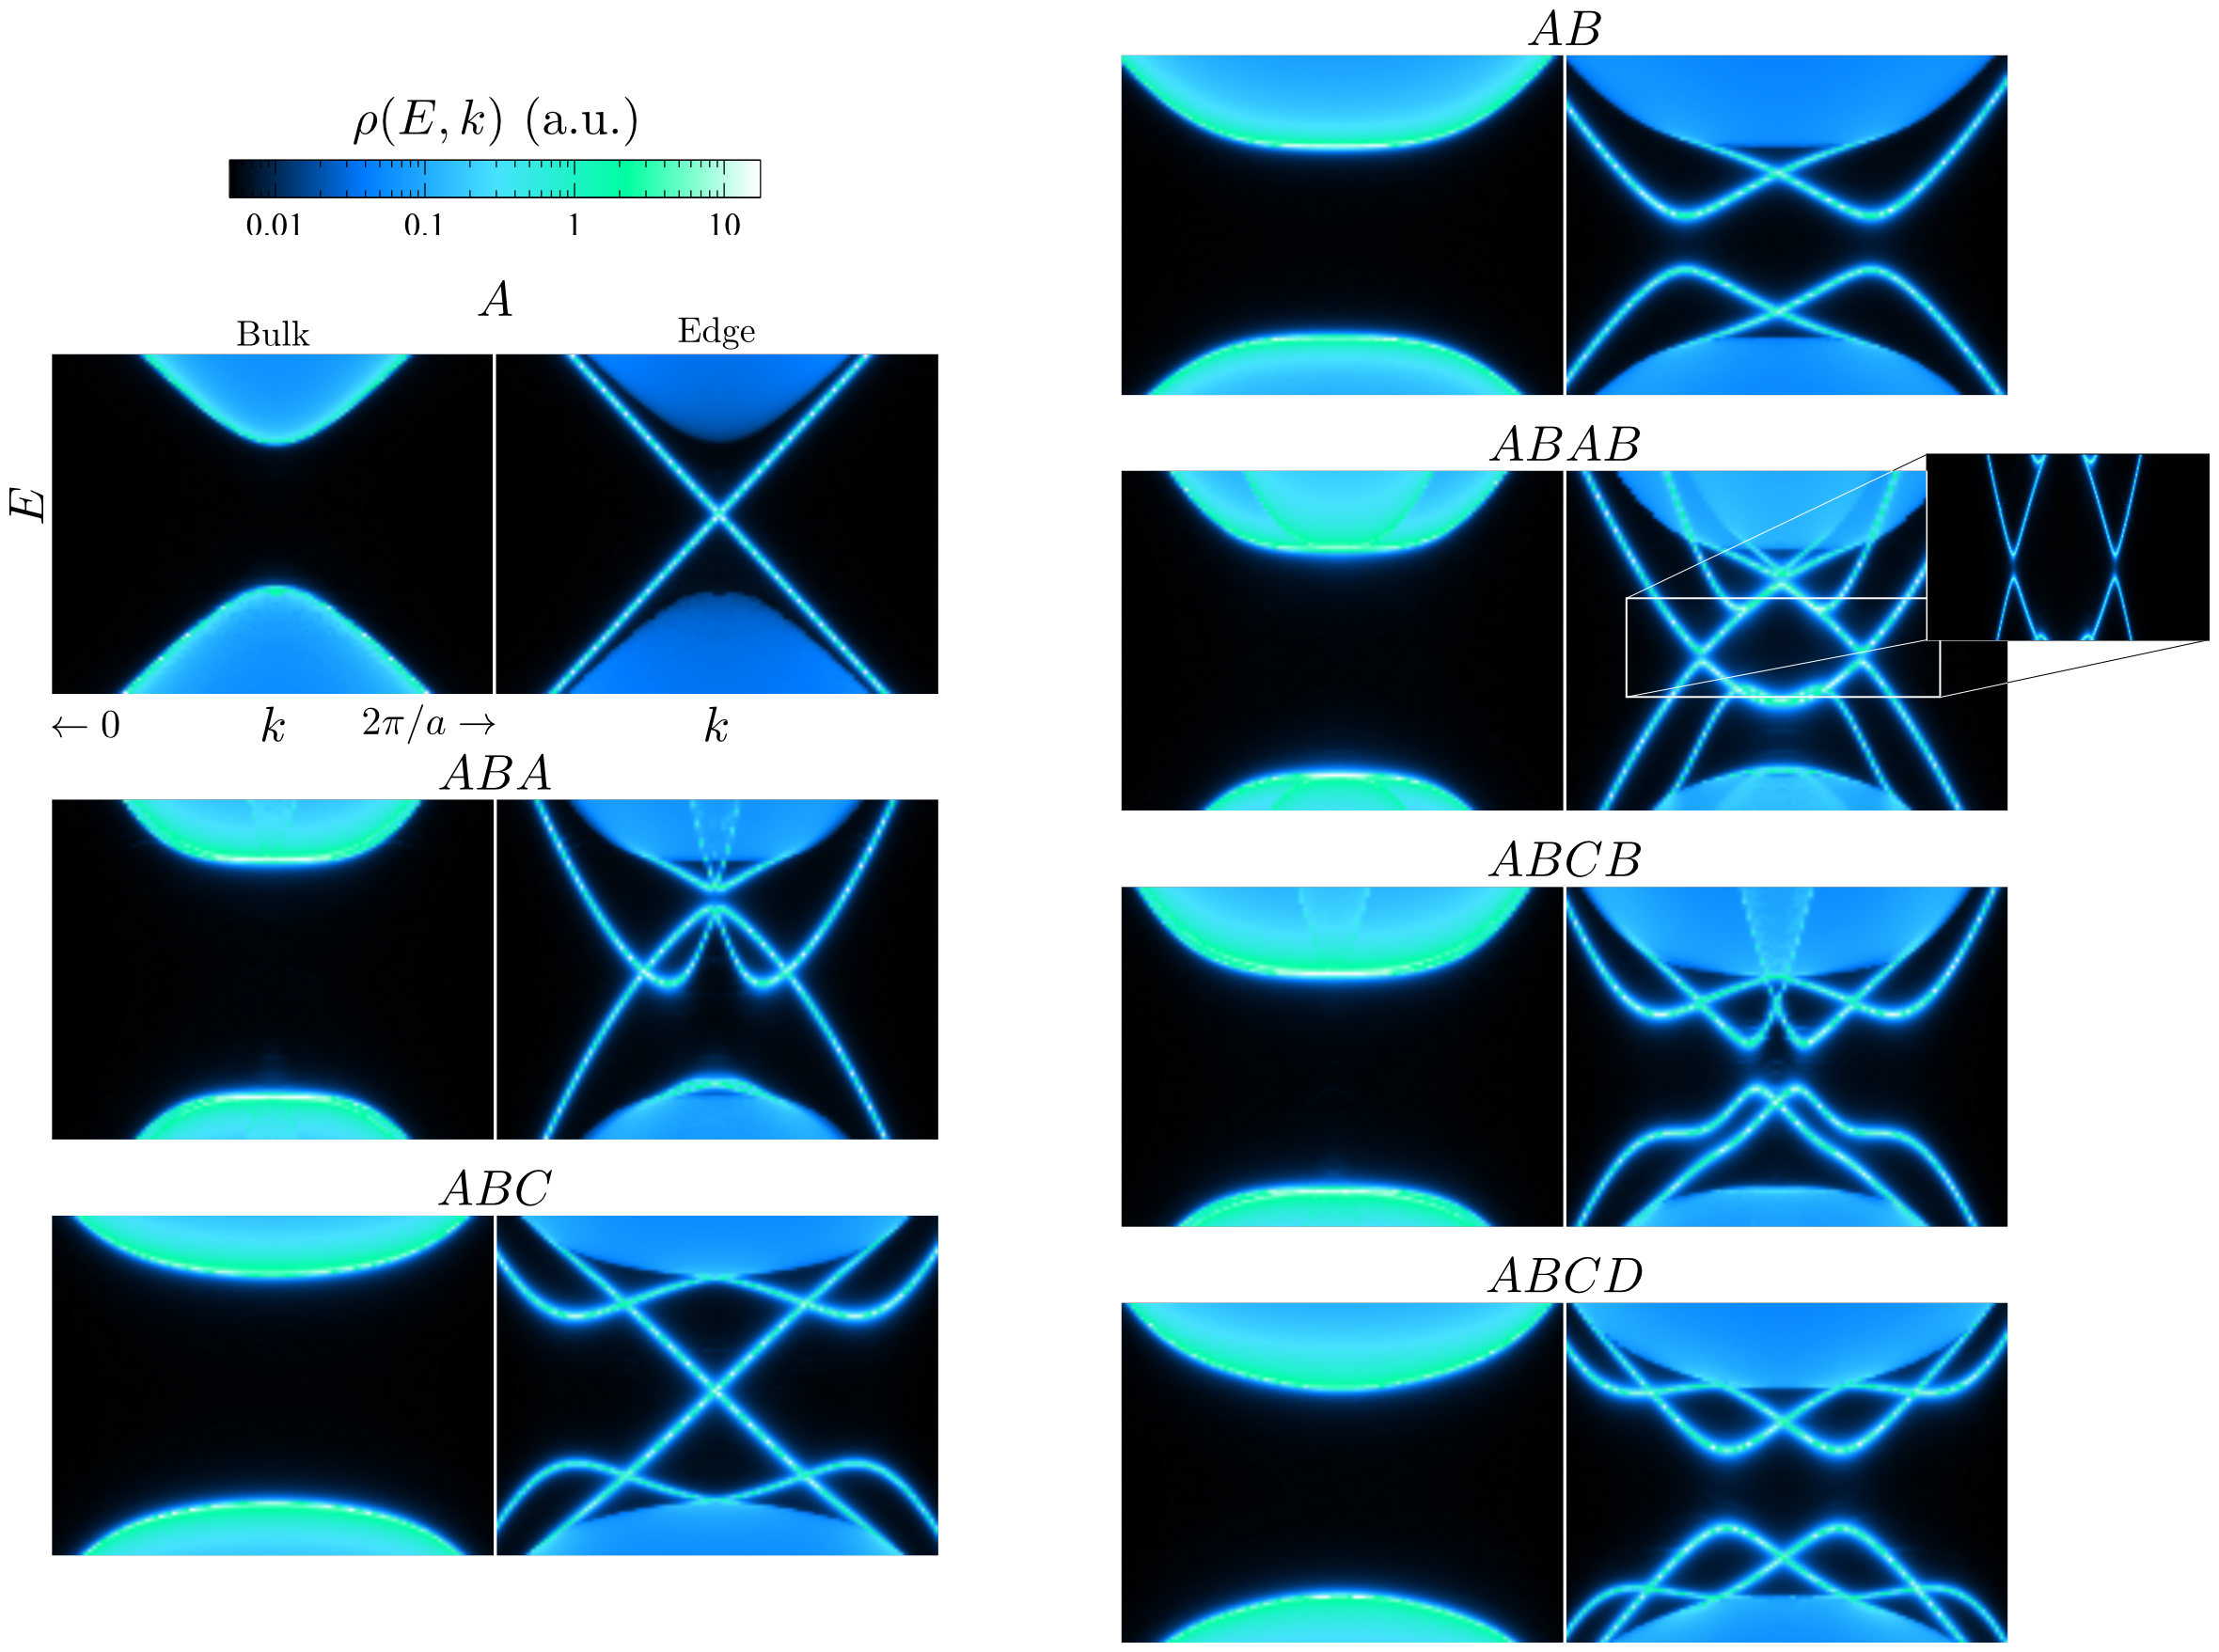
\includegraphics[width=\textwidth]{chapter04/figures/dyson.png}
% \end{center}
% \end{minipage}
\caption{For each structure bulk and edge \ac{dos} (left and right panel respectively).
Gapless edge states appear only when an odd number of layers is considered independently of the stacking used.}
\label{DOSdyson}
\end{figure*}


The surface Green function of this  block tridiagonal semi-infinite matrix can be  written as:
\begin{equation}
G^{edge}(E,k_{||}) =
\left[E+i\epsilon-H_0(k_{||})-\Sigma_{R}(k_{||})-\Sigma_{H}(k_{||})\right]^{-1}
\end{equation}
where $\Sigma_{R}(k_{||})$ is a self-energy that accounts for the coupling to the semi-infinite crystal,
$\Sigma_{H}(k_{||})$ is the self-energy due to its interaction with the $H$ atoms included to get rid of the dangling bonds and $\epsilon$ a small analytic continuation.

The self-energy $\Sigma_{R}$ can be calculated employing a recursive Green's function method that leads to the following coupled equations
\begin{eqnarray}
\nonumber \Sigma_{R}(E,k_{||})&=& V_{R}(k_{||})g_{R}(E,k_{||})V^{\dagger}_{R}(k_{||})
\\
g_{R}(E,k_{||}) &=& \left[E-H_0(k_{||}) -\Sigma_{R}(E,k_{||})\right]^{-1}
\end{eqnarray}

The $\Sigma_{H}(k_{||})$ is calculated just as an additional iteration to the self-consistent calculation with the appropriate value for the hoppings $C-H$.

For a given $k_{||}$ we compute the \ac{dos} using
\begin{equation}
 \rho(E,k_{||}) = -\frac{1}{\pi} Im[G^{edge}(E,k_{||})]
\end{equation}
Using a similar  approach we can also obtain the bulk \ac{dos}  calculating the bulk Green function by recursion.

In figure~\ref{DOSdyson} we show the \ac{dos} for both bulk and edge for all the stackings as a contour plot in the $k_{||},E$ plane. For each stacking the left panel shows the bulk \ac{dos}, which are gaped for all the stackings and the right panel shows the edge states.  The calculations are done for a rather large value of $\lambda=\SI{2}{\eV}$. The first thing to  notice is that, for such large values of $\lambda$, all the structures have edge states. However, only in the case of odd $N$, shown in the left column, the in-gap states are gapless.  This is a necessary condition in order to have a \ac{qshi}.  In contrast,  all systems with even $N$ have edge states with a gap. Thereby, they are definitely not in the \ac{qsh} phase, validating
 equation~\eqref{trivial}. Therefore, we conclude that odd  $N$ graphene stacks are \ac{qshi} and even $N$ are trivial insulators. In all cases, the gap opened by \ac{soc} is quite small.



%%%%%%%%%%%%%%%%%%%%%%%%%%%%%%%%%%%%%%%%%%%%%%%%%%%%%%%%%%%%%%%%%%%%%%%%%%%%%%%%
\subsection{Heterogeneous multilayers}
\label{Heterogeneous}
In the previous section we have seen that for homogeneous multilayers the gap opened by \ac{soc} has the same magnitude than for the monolayer. Thereby, homogeneous multilayers of graphene  would not improve the prospects for observation of the \ac{qsh} phase compared to the monolayer. We thus explore the case of a heterogeneous multilayer. This is motivated in part by recent experiments~\cite{Avsar2014} that seem to indicate an enhancement of the \ac{soc} interaction in graphene due to proximity to WS$_2$, a trivial semiconductor with quite large \ac{soc} and no inversion symmetry. There has also been plenty of work studying the enhancement of \ac{soc} interaction in graphene due to proximity to heavy metals~\cite{Zhang2014a}. However, it would be much more interesting if graphene could be driven into a \ac{qsh} phase by proximity to an insulator, so that the only conducting channels would be only at the edges of graphene.

Density functional calculations show~\cite{Kaloni2014} that a topological band-gap opens in graphene on top of both $WS_2$ and $WSe_2$, two widely studied two dimensional \acp{tmd}.  The magnitude of this gap is in the range of a few meV, i.e.,  two or  three orders of magnitude larger than  the intrinsic \ac{soc} gap.

%~~~~~~~~~~~~~~~~~~~~~~~~~~ FIGURE ~~~~~~~~~~~~~~~~~~~~~~~~~%
\begin{figure}[hbt]
 \centering
  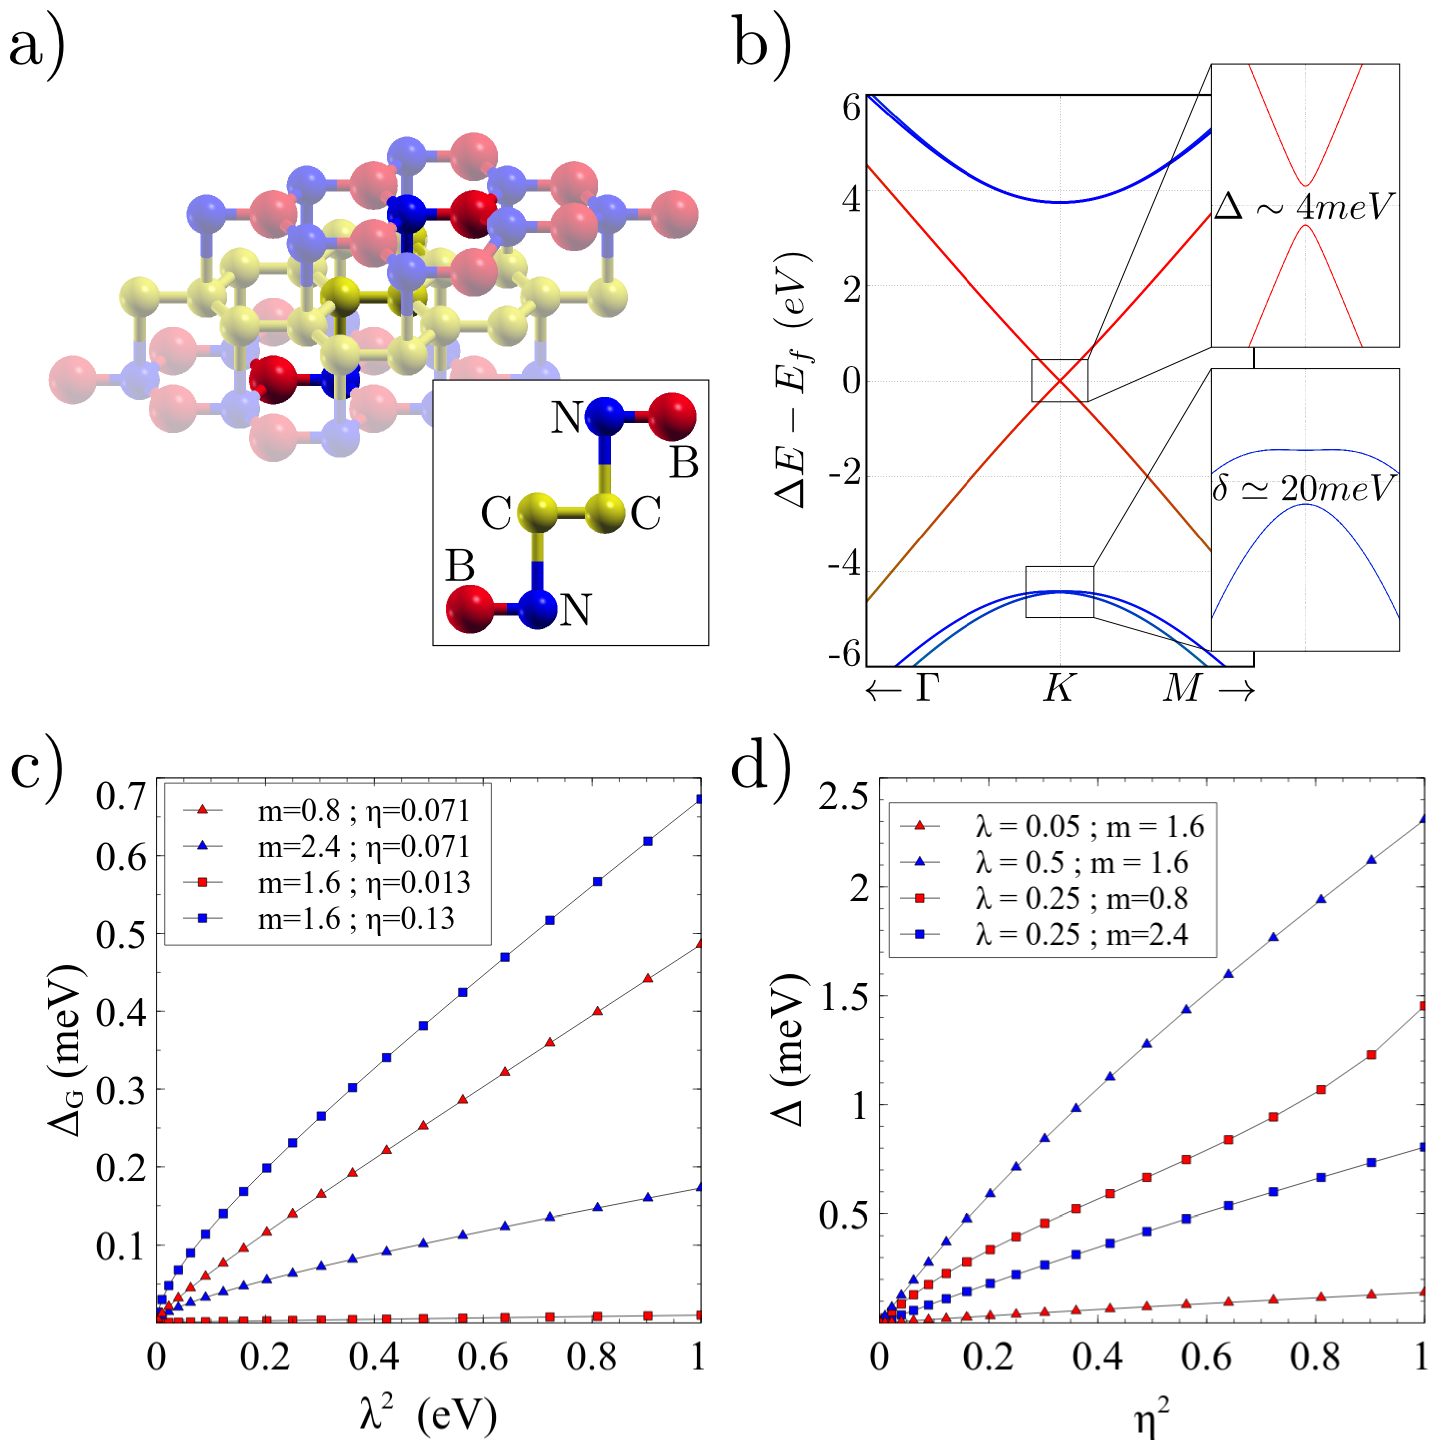
\includegraphics{chapter04/figures/encapsulated.png}
\caption{Panel $a)$ shows the structure of the heterostructure considered.
Panels (b,c,d) show the dependence of the induced gap in graphene due to the proximity of the encapsulating layers. In panel $b)$ it can be seen that the gap is proportional to $\lambda^{2}$ and this estimation gets better as the gap of insulating layers gets bigger. Panel $b)$ shows how the interlayer coupling $\eta$ produces the expected effect, for small interlayer coupling the induced gap is small but it grows quickly as $\eta$ increases. Panel $c)$ shows the dependence of the induced gap with the sublattice imbalance}
\label{induced}
\end{figure}
%~~~~~~~~~~~~~~~~~~~~~~~~~~~~~~~~~~~~~~~~~~~~~~~~~~~~~~~~~~~%

Here we propose a toy model to understand the opening of a non-trivial gap due to proximity to a trivial insulator with strong \ac{soc}.
For that matter, we take graphene encapsulated between two monolayers of a trivial semiconductor with strong \ac{soc} and broken inversion symmetry.   Specifically, the structure of  these adjacent monolayers is that of a $BN$-like crystal (see figure~\ref{induced}(a)).   The choice of the stacking is such that, globally, the structure has inversion symmetry. Otherwise,  a trivial band gap would be opened by proximity~\cite{Giovannetti2007}.

The $BN$-like crystal is described with the same interatomic \ac{sk} parameters than graphene, but very different on-site parameters. In particular we assume a large \ac{soc} $\lambda$ and a staggered potential $\pm m$ that breaks inversion symmetry of the top and bottom layers.
Since we are interested in the proximity effect, we turn off the atomic \ac{soc} of the graphene layer.
As in the case of the homogeneous multilayers, the interlayer coupling is characterized by the dimensionless parameter $\eta$.   In this case we impose
zero \ac{soc} for the graphene layer, in order to study the proximity effect.   For $\eta=0$ the bands of this system would be the superposition of those of the top and bottom insulators, with gap $2m$, and the bands of graphene, whose Dirac cones would lie inside the gap.  Broadly speaking, this picture remains the same as the interlayer coupling is turned on.    Interestingly, a non-trivial gap $\Delta$  opens in the Dirac cones only when $\eta\neq 0$ and $\lambda\neq 0$.  We have verified that this gap satisfies the  scaling
\begin{equation}
\Delta \propto \frac{\lambda \eta^2}{m^{2}}
\label{wcoupling}
\end{equation}
in the limit of small $\lambda$, $\eta$ and $m^{-1}$. This results implies that graphene can borrow \ac{soc} from a neighbor trivial insulator layer via interlayer coupling. Using the method of the TRIM  we have verified that this insulator has $Z_2=(-1)^{\nu}=-1$, and is therefore topologically non-trivial.

The magnitude of the proximity effect away from the weak coupling limit of eq. \eqref{wcoupling} is shown in figures \ref{induced}.  We study the dependence of the proximity gap $\Delta$ as a function of both the \ac{soc} $\lambda$ and the interlayer coupling $\eta$ for two values of the encapsulating layer  staggered potential $m$. It is apparent that, taking $m=\SI{2.0}{\eV}$ (a trivial gap $\sim\SI{1.5}{\eV}$) and $\lambda \simeq \SI{0.25}{\eV}$, values in line with those of 2D \ac{tmd}, the proximity gap is in the order of
 $\sim\SI{1}{\meV}$, similar to the \ac{dft} results. Therefore, our model provides a reasonable justification of the \ac{dft} computations, which are certainly more complete.

Our  toy model does not capture some probably important features of real heterogeneous multilayers.  For instance,
the interlayer interaction  could break inversion symmetry which is expected to open a trivial gap.  In addition,
the geometry of our encapsulating  layers was  chosen to minimize the size of the unit cell, rather than to describe a real material.  In general, the coupling of graphene to other 2D crystals will imply a new length scale, given by the size of the new unit cell. In this setup, the inversion symmetry breaking could average out.


% \section{Graphene bilayer}
%%%%%%%%%%%%%%%%%%%%%%%%%%%%%%%%%%%%%%%%%%%%%%%%%%%%%%%%%%%%%%%%%%%%%%%%%%%%%%%%
% \section{Conclusions}\label{conclus}
% We have studied the quantum spin Hall phase in multilayer graphene and in graphene encapsulated by a trivial semiconductor. In the case of multilayer graphene we find that only the stacks with an odd number of layers are quantum spin Hall insulators. However, the size of the gap is the same than for a monolayer, and thereby, most likely too small to be detected experimentally.
% In contrast, we propose a toy model for  graphene encapsulated between two semiconducting layers with strong SOC and a trivial gap. Our model shows that  a non-trivial gap can be opened in graphene whose magnitude is controlled by the atomic spin orbit coupling of the adjacent layers. Our model provides a qualitative understanding of recent \ac{dft} calculations~\cite{Zhang2014a} as well as recent experimental work~\cite{Avsar2014} and shows a promising route to observe the quantum spin Hall phase in graphene.
%%%%%%%%%%%%%%%%%%%%%%%%%%%%%%%%%%%%%%%%%%%%%%%%%%%%%%%%%%%%%%%%%%%%%%%%%%%%%%%%
%%%%%%%%%%%%%%%%%%%%%%%%%%%%%%%%%%%%%%%%%%%%%%%%%%%%%%%%%%%%%%%%%%%%%%%%%%%%%%%%
